%% Module 2 beamer/knitr slides
%% Biostatistics in Practice workshop, January 2014
%% Nicholas Reich: nick [at] schoolph.umass.edu


\documentclass[table]{beamer}\usepackage[]{graphicx}\usepackage[]{color}
% maxwidth is the original width if it is less than linewidth
% otherwise use linewidth (to make sure the graphics do not exceed the margin)
\makeatletter
\def\maxwidth{ %
  \ifdim\Gin@nat@width>\linewidth
    \linewidth
  \else
    \Gin@nat@width
  \fi
}
\makeatother

\definecolor{fgcolor}{rgb}{0.345, 0.345, 0.345}
\newcommand{\hlnum}[1]{\textcolor[rgb]{0.686,0.059,0.569}{#1}}%
\newcommand{\hlstr}[1]{\textcolor[rgb]{0.192,0.494,0.8}{#1}}%
\newcommand{\hlcom}[1]{\textcolor[rgb]{0.678,0.584,0.686}{\textit{#1}}}%
\newcommand{\hlopt}[1]{\textcolor[rgb]{0,0,0}{#1}}%
\newcommand{\hlstd}[1]{\textcolor[rgb]{0.345,0.345,0.345}{#1}}%
\newcommand{\hlkwa}[1]{\textcolor[rgb]{0.161,0.373,0.58}{\textbf{#1}}}%
\newcommand{\hlkwb}[1]{\textcolor[rgb]{0.69,0.353,0.396}{#1}}%
\newcommand{\hlkwc}[1]{\textcolor[rgb]{0.333,0.667,0.333}{#1}}%
\newcommand{\hlkwd}[1]{\textcolor[rgb]{0.737,0.353,0.396}{\textbf{#1}}}%
\let\hlipl\hlkwb

\usepackage{framed}
\makeatletter
\newenvironment{kframe}{%
 \def\at@end@of@kframe{}%
 \ifinner\ifhmode%
  \def\at@end@of@kframe{\end{minipage}}%
  \begin{minipage}{\columnwidth}%
 \fi\fi%
 \def\FrameCommand##1{\hskip\@totalleftmargin \hskip-\fboxsep
 \colorbox{shadecolor}{##1}\hskip-\fboxsep
     % There is no \\@totalrightmargin, so:
     \hskip-\linewidth \hskip-\@totalleftmargin \hskip\columnwidth}%
 \MakeFramed {\advance\hsize-\width
   \@totalleftmargin\z@ \linewidth\hsize
   \@setminipage}}%
 {\par\unskip\endMakeFramed%
 \at@end@of@kframe}
\makeatother

\definecolor{shadecolor}{rgb}{.97, .97, .97}
\definecolor{messagecolor}{rgb}{0, 0, 0}
\definecolor{warningcolor}{rgb}{1, 0, 1}
\definecolor{errorcolor}{rgb}{1, 0, 0}
\newenvironment{knitrout}{}{} % an empty environment to be redefined in TeX

\usepackage{alltt}


%       ************************************************
%       **        LaTeX preamble to be used with all 
%	**        statsTeachR labs/handouts.
%
%	Author: Nicholas G Reich
%	Last modified: 14 January 2014
%	************************************************

% \documentclass[table]{beamer}

%	Set theme (a nice plain one)
\usetheme{Malmoe}

%	Use named colors, set main color of theme
%		to match Web site color:
\definecolor{MainColor}{RGB}{10, 74, 109}
\colorlet{MainColorMedium}{MainColor!50}
\colorlet{MainColorLight}{MainColor!20}
\usecolortheme[named=MainColor]{structure} 

%	For tables
%[dvipsnames] [table]
\usepackage{xcolor}

%% calling tabu.sty, assuming a particular directory structure
\usepackage{../../slide-includes/tabu}	% Even fancier than tabulary
\usepackage{multirow}

%	Just for the degree symbol
\usepackage{textcomp}

%	Get rid of footline (page, author, etc. on each slide)
\setbeamertemplate{footline}{}
%	Get rid of navigation buttons
\setbeamertemplate{navigation symbols}{}

%	Make footnotes not ugly
\usepackage{hanging}
\setbeamertemplate{footnote}{\raggedright\hangpara{1em}{1}\makebox[1em][l]{\insertfootnotemark}\footnotesize\insertfootnotetext\par}

%	Text style for code snippets inline in text:
\newcommand{\codeInline}[1]{\texttt{#1}}

%	Text style for emphasis stronger than \emph:
%		(Note, this doesn't toggle the way \emph does.
%			(Note, this can be done, didn't seem worth the trouble.))
\newcommand{\strong}[1]{{\bfseries{#1}}}


%        ******	Define title page	**********************
\setbeamertemplate{title page}{
	{\color{MainColor}
	% There must be a better way than this -vspace at
	%	 the top and bottom of the page to reduce the 
	%	 bottom margin, but I can't find one that works.
	\vspace{-6em}

% 	% Go to a lot of trouble to get the title in a
% 	%	nice box, since customizing a beamer block
% 	%	does not entirely work here (I don't know why)
	\newlength{\titleBoxWidth}
	\setlength{\titleBoxWidth}{\textwidth}
	\addtolength{\titleBoxWidth}{-2.0em}
	\setlength{\fboxsep}{1.0em}
	\setlength{\fboxrule}{0pt}
	\fcolorbox{MainColor!25}{MainColor!25}{
		\parbox{\titleBoxWidth}{
			\raggedright
			\LARGE\textbf{\inserttitle}
		}	% end parbox
	}	% end fcolorbox

	\vfill
	\small{Author: \insertauthor}
	\vspace{\baselineskip}

	\small{\Course}

	\small{\Instructor}
	\vspace{\baselineskip}

	%\small{\emph{This material is part of the \strong{statsTeachR} project}}

	\vspace{0.33\baselineskip}\scriptsize{\emph{\LicenseText}}


		\vspace{-15em}

	}	% end color
	\clearpage
}	% end define title page

%        The following variables are assumed by the standard preamble:
%	Global variable containing module name:
\title{Using splines in regression}
%	Global variable containing module shortname:
%		(Currently unused, may be used in future.)
\newcommand{\ModuleShortname}{MLR}
%	Global variable containing author name:
\author{Nicholas G Reich, adapted from content by Andrea Foulkes}
%	Global variable containing text of license terms:
\newcommand{\LicenseText}{Made available under the Creative Commons Attribution-ShareAlike 3.0 Unported License: http://creativecommons.org/licenses/by-sa/3.0/deed.en\_US }
%	Instructor: optional, can leave blank.
%		Recommended format: {Instructor: Jane Doe}
\newcommand{\Instructor}{}
%	Course: optional, can leave blank.
%		Recommended format: {Course: Biostatistics 101}
\newcommand{\Course}{}

\input{../../slide-includes/shortcuts}
\usepackage{bbm}
\hypersetup{colorlinks=TRUE, urlcolor=blue}

%%%%%%%% IMPORTANT -- MUST HAVE [fragile] for some/all frames chunks to have output work correctly.
\IfFileExists{upquote.sty}{\usepackage{upquote}}{}
\begin{document}




\begin{frame}[plain]
        \titlepage
\end{frame}




%%%%%%%%%%%%%%%%%%%%%%%%%%%%%%%%%%%%%%%%%%

\begin{frame}{Today's Lecture}

\bi
    \myitem Assessing model accuracy
    \myitem Overfitting
    \myitem Fitting smooth curves to data
\ei

\vspace{2em}

More info: 
\bi
    \myitem For more gory details: {\em Intro to Statistical Learning} Chapter 7
\ei


\end{frame}

%%%%%%%%%%%%%%%%%%%%%%%%%%%%%%%%%%%%%%%%%%

\begin{frame}{Assessing model accuracy: Regression setting}
\begin{itemize}
\item The {\color{orange} mean squared error (MSE)} is the most commonly used measure of the performance of a statistical learning method in the regression setting:
%
\begin{eqnarray*}
MSE = \frac{1}{n} \sum_{i=1}^n \left(y_i -\hat y_i\right)^2
\end{eqnarray*}

\bigskip
\item The MSE will be small if the observed and predicted responses are close to one another, and it will be large if these differ substantially, in at least some instances.
\end{itemize}
\end{frame}


%%%%%%%%%%%%%%%%%%%%%%%%%%%%%%%%%%%%%%%%%%

\begin{frame}{Low MSE is not always a good thing!}
\begin{itemize}
  \item Which color line/model do you think has the lowest MSE?
  \item Which color line/model would you trust the most to predict a new observation?
\end{itemize}

\centerline{
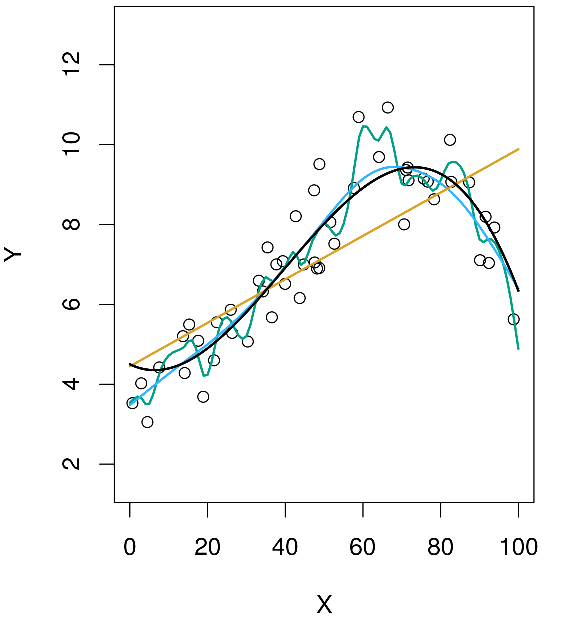
\includegraphics[scale=.6,angle=0]{figure-static/2_9-half.pdf}
}


\end{frame}

%%%%%%%%%%%%%%%%%%%%%%%%%%%%%%%%%%%%%%%%%%

\begin{frame}{How to find the ``sweet spot''?}
\begin{itemize}
  \item Ideally, your model should predict observations well in your dataset (``in-sample'') and in a new dataset (``out-of-sample''). 
  \item While this is not often possible in practice, ideally the new dataset should be completely separately collected from the initial dataset.
  \item Example 1: a study done by investigators at Institution A shows that in a sample of 100 cancer patients, a specific set of commonly collected biomarkers accurately classified cancer patients based on severity of outcome at 1 year follow-up. What would be a good replication study?
  % \item Example 2: using photos from a common social media platform, authors claimed that their face recognition algorithm could accurately predict the sexual orientation of individuals based solely on the photo. What would be a good replication study?
\end{itemize}
\end{frame}

%%%%%%%%%%%%%%%%%%%%%%%%%%%%%%%%%%%%%%%%%%

\begin{frame}{Often, an `internal` test sample is used}
\begin{itemize}
  \item In general, we are interested in the accuracy of the predictions that we obtain when we apply our method to previously unseen data $\rightarrow$  called the {\color{violet} test sample}. \\
  \item Often, obtaining an external validation or testing dataset is infeasible or expensive.
  \item In these cases, investigators may set aside a portion of the observations from the original dataset as a {\color{violet} test sample}.
  \item Test samples can be particularly useful in diagnosing whether your model was ``overfit`` to the particular features of the training dataset.
\end{itemize}
\end{frame}


%%%%%%%%%%%%%%%%%%%%%%%%%%%%%%%%%%%%%%%%%%

\begin{frame}[fragile]{Hands-on example: FEV dataset}

The FEV dataset describes a sample of 654 youths, aged 3 to 19, in the area of East Boston during middle to late 1970's. Data includes the following variables (among others)

\begin{itemize}
  \item fev - forced expiratory volume, a measure of lung capacity and strength (in liters)
  \item height (in inches)
\end{itemize}

\scriptsize
\begin{knitrout}\footnotesize
\definecolor{shadecolor}{rgb}{0.969, 0.969, 0.969}\color{fgcolor}\begin{kframe}
\begin{alltt}
\hlkwd{library}\hlstd{(}\hlstr{"Hmisc"}\hlstd{)}
\hlkwd{getHdata}\hlstd{(FEV)}
\hlkwd{head}\hlstd{(FEV)}
\end{alltt}
\begin{verbatim}
##     id age   fev height    sex              smoke
## 1  301   9 1.708   57.0 female non-current smoker
## 2  451   8 1.724   67.5 female non-current smoker
## 3  501   7 1.720   54.5 female non-current smoker
## 4  642   9 1.558   53.0   male non-current smoker
## 5  901   9 1.895   57.0   male non-current smoker
## 6 1701   8 2.336   61.0 female non-current smoker
\end{verbatim}
\end{kframe}
\end{knitrout}

\end{frame}

%%%%%%%%%%%%%%%%%%%%%%%%%%%%%%%%%%%%%%%%%%

\begin{frame}[fragile]{Creating an FEV test sample}

\scriptsize
\begin{knitrout}\footnotesize
\definecolor{shadecolor}{rgb}{0.969, 0.969, 0.969}\color{fgcolor}\begin{kframe}
\begin{alltt}
\hlkwd{set.seed}\hlstd{(}\hlnum{756}\hlstd{)}  \hlcom{## so we all get the same result}
\hlstd{idx_test} \hlkwb{<-} \hlkwd{sample}\hlstd{(}\hlnum{1}\hlopt{:}\hlkwd{nrow}\hlstd{(FEV),} \hlkwc{size}\hlstd{=}\hlnum{200}\hlstd{)} \hlcom{## 200 test observations}
\hlstd{fev_train} \hlkwb{<-} \hlstd{FEV[}\hlopt{-}\hlstd{idx_test,]}    \hlcom{## removing all test observations }
\hlstd{fev_test} \hlkwb{<-} \hlstd{FEV[idx_test,]}      \hlcom{## leaving all test observations}
\hlkwd{ggplot}\hlstd{(fev_train,} \hlkwd{aes}\hlstd{(height, fev))} \hlopt{+} \hlkwd{geom_point}\hlstd{()} \hlopt{+}
  \hlkwd{geom_smooth}\hlstd{(}\hlkwc{method}\hlstd{=}\hlstr{"lm"}\hlstd{,} \hlkwc{se}\hlstd{=}\hlnum{FALSE}\hlstd{)}
\end{alltt}
\end{kframe}

{\centering 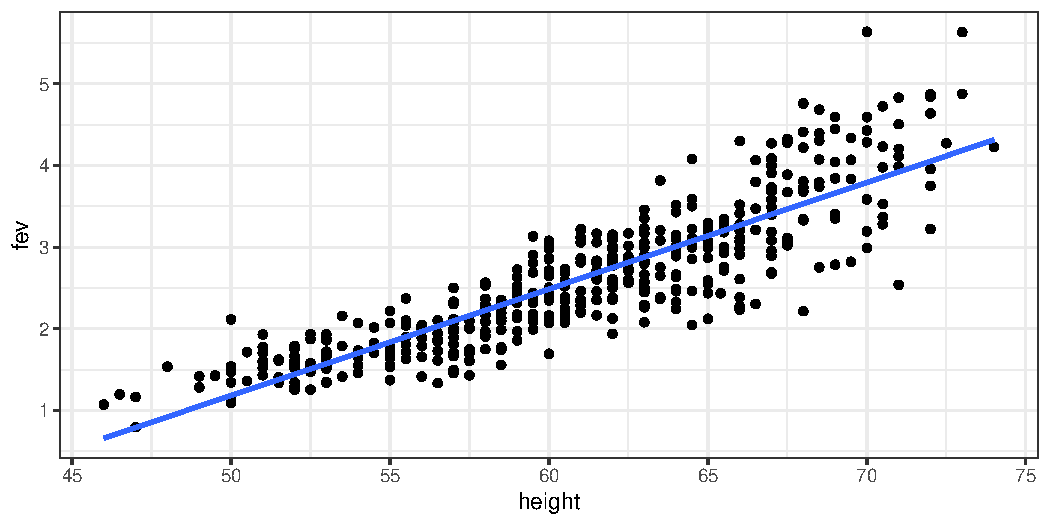
\includegraphics[width=\maxwidth]{figs/beamer-unnamed-chunk-2-1} 

}



\end{knitrout}

\end{frame}

%%%%%%%%%%%%%%%%%%%%%%%%%%%%%%%%%%%%%%%%%%

\begin{frame}[fragile]{Using a smooth model for $fev \sim height$}

Let's fit a model to the data that can capture some of what appears to be a non-linear relationship between height and fev.

The {\tt ns()} function in the splines package uses a "natural spline" to model a flexible, non-linear relationship bewteen a covariate and an outcome by splicing together polynomial functions. The larger the ``degrees of freedom'' ({\tt df}) parameter is, the more functions it pieces together and therefore the more wiggly the fitted model becomes. 

\scriptsize
\begin{knitrout}\footnotesize
\definecolor{shadecolor}{rgb}{0.969, 0.969, 0.969}\color{fgcolor}\begin{kframe}
\begin{alltt}
\hlkwd{library}\hlstd{(splines)}
\hlstd{spline_mdl} \hlkwb{<-} \hlkwd{lm}\hlstd{(fev} \hlopt{~} \hlkwd{ns}\hlstd{(height,} \hlkwc{df} \hlstd{=} \hlnum{4}\hlstd{),} \hlkwc{data}\hlstd{=fev_train)}
\end{alltt}
\end{kframe}
\end{knitrout}

\end{frame}

%%%%%%%%%%%%%%%%%%%%%%%%%%%%%%%%%%%%%%%%%%

\begin{frame}[fragile]{Visualizing the smooth model}


\scriptsize
\begin{knitrout}\footnotesize
\definecolor{shadecolor}{rgb}{0.969, 0.969, 0.969}\color{fgcolor}\begin{kframe}
\begin{alltt}
\hlstd{spline_x_vals} \hlkwb{<-} \hlkwd{seq}\hlstd{(}\hlnum{45}\hlstd{,} \hlnum{75}\hlstd{,} \hlkwc{by}\hlstd{=}\hlnum{1}\hlstd{)}
\hlstd{spline_y_vals} \hlkwb{<-} \hlkwd{predict}\hlstd{(spline_mdl,}
  \hlkwc{newdata} \hlstd{=} \hlkwd{data.frame}\hlstd{(}\hlkwc{height}\hlstd{=spline_x_vals))}
\hlkwd{ggplot}\hlstd{()} \hlopt{+}
  \hlkwd{geom_point}\hlstd{(}\hlkwd{aes}\hlstd{(}\hlkwc{x}\hlstd{=height,} \hlkwc{y}\hlstd{=fev),} \hlkwc{data}\hlstd{=fev_train)} \hlopt{+}
  \hlkwd{geom_line}\hlstd{(}\hlkwd{aes}\hlstd{(}\hlkwc{x} \hlstd{= spline_x_vals,} \hlkwc{y}\hlstd{=spline_y_vals),} \hlkwc{color}\hlstd{=}\hlstr{"red"}\hlstd{)}
\end{alltt}
\end{kframe}

{\centering 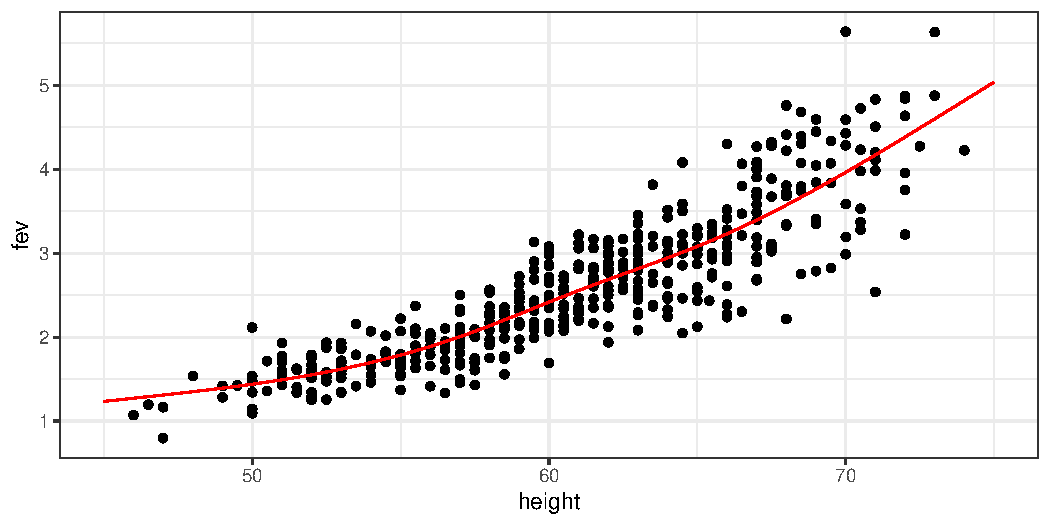
\includegraphics[width=\maxwidth]{figs/beamer-unnamed-chunk-4-1} 

}



\end{knitrout}

\end{frame}


%%%%%%%%%%%%%%%%%%%%%%%%%%%%%%%%%%%%%%%%%%

\begin{frame}[fragile]{Find the Goldilocks zone!}

That model looks good, but how to we know what degree of smoothness is just the right amount? We can compare MSE between our training and our test set for different levels of smoothness.

\scriptsize
\begin{knitrout}\footnotesize
\definecolor{shadecolor}{rgb}{0.969, 0.969, 0.969}\color{fgcolor}\begin{kframe}
\begin{alltt}
\hlstd{fev_train}\hlopt{$}\hlstd{spline_preds} \hlkwb{<-} \hlkwd{predict}\hlstd{(spline_mdl)}
\hlstd{fev_test}\hlopt{$}\hlstd{spline_preds} \hlkwb{<-} \hlkwd{predict}\hlstd{(spline_mdl,} \hlkwc{newdata} \hlstd{= fev_test)}
\hlstd{( mse_train} \hlkwb{<-} \hlkwd{mean}\hlstd{((fev_train}\hlopt{$}\hlstd{fev} \hlopt{-} \hlstd{fev_train}\hlopt{$}\hlstd{spline_preds)}\hlopt{^}\hlnum{2}\hlstd{) )}
\end{alltt}
\begin{verbatim}
## [1] 0.1632517
\end{verbatim}
\begin{alltt}
\hlstd{( mse_test} \hlkwb{<-} \hlkwd{mean}\hlstd{((fev_test}\hlopt{$}\hlstd{fev} \hlopt{-} \hlstd{fev_test}\hlopt{$}\hlstd{spline_preds)}\hlopt{^}\hlnum{2}\hlstd{) )}
\end{alltt}
\begin{verbatim}
## [1] 0.1816097
\end{verbatim}
\end{kframe}
\end{knitrout}

\end{frame}
%%%%%%%%%%%%%%%%%%%%%%%%%%%%%%%%%%%%%%%%%%

\begin{frame}[fragile]{With your group}

\begin{itemize}
\item In your breakout rooms, pick a set of {\tt df} to test as a group. Work together to make sure that at least one {\tt df} is run on everyone's computer. 
\item Compile a dataset on the note-catcher with the {\tt df} value and the associated MSEs for both the training and testing samples. 
\item Discuss your results as a table and decide on an optimal {\tt df} to choose.
\end{itemize}

\end{frame}

%%%%%%%%%%%%%%%%%%%%%%%%%%%%%%%%%%%%%%%%%%

\begin{frame}{Using a test sample avoids ``overfitting''}
\begin{itemize}
  \item A good rule of thumb of a good model is that it will generalize to another setting.
  \item Therefore, a good model is one that {\bf minimizes the test sample MSE.}
  \item The mean squared error will always get lower with the training sample as we add more features to our model.
  \item {\color{orange} Overfitting} refers to the situation in which a less complex or ``wiggly'' model would result in a smaller test sample MSE.
\end{itemize}
\end{frame}

%%%%%%%%%%%%%%%%%%%%%%%%%%%%%%%%%%%%%%%%%%


\begin{frame}{MSE: learning versus test sample}
\centerline{
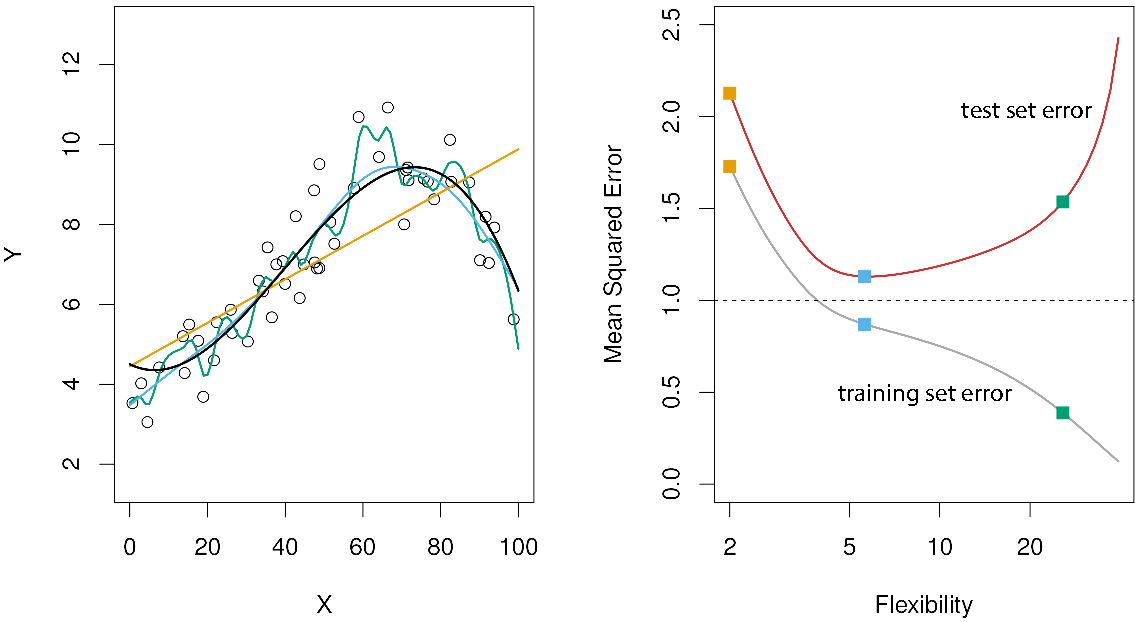
\includegraphics[scale=.6,angle=0]{figure-static/2_9-all.pdf}
}

Figure 2.9 from ISL. Black line is the true relationship from which data are simulated
\end{frame}

\begin{frame}{MSE: learning versus test sample}
\centerline{
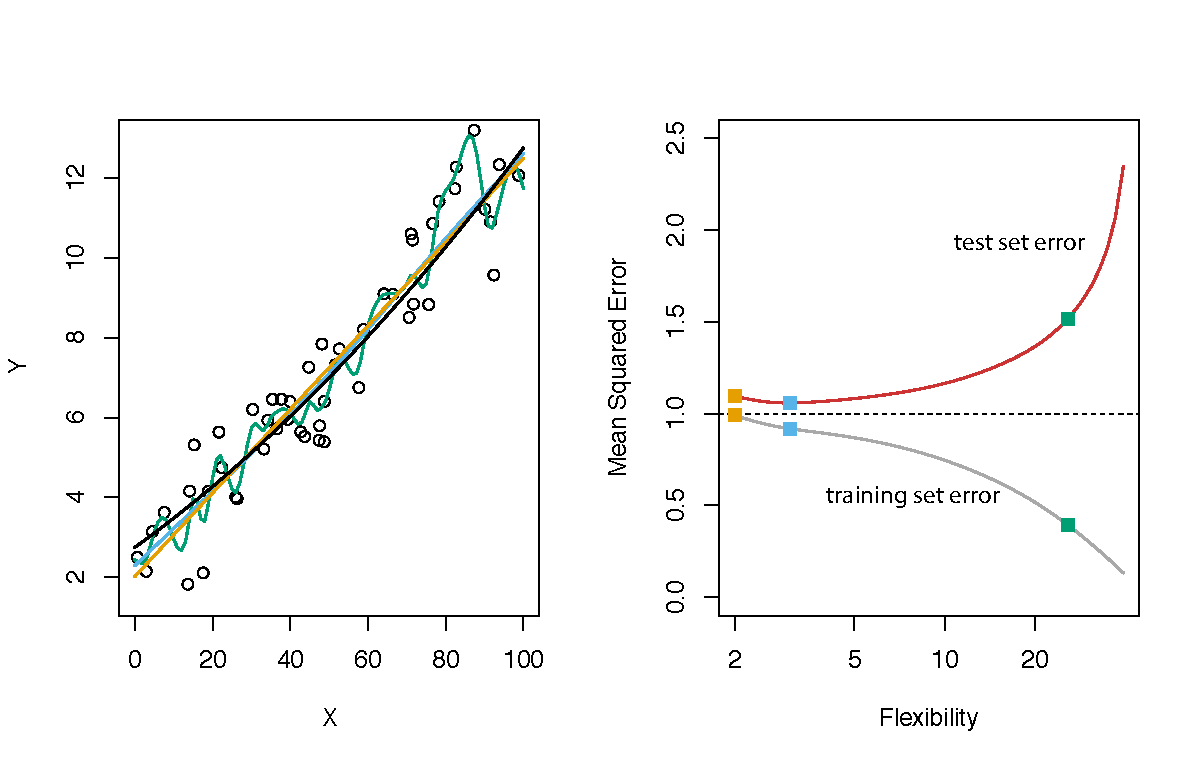
\includegraphics[scale=.6,angle=0]{figure-static/2_10.pdf}
}
Figure 2.10 from ISL.

\end{frame}


\begin{frame}{Summary}

Validating potential models on external data is critical to understanding how well your model will generalize to another dataset.

\end{frame}



\end{document}
